\pdfoutput=1
%\documentclass[handout]{beamer}
\documentclass[red,handout,professionalfont]{beamer}
% \documentclass[red,professionalfont]{beamer}
\usepackage{multimedia}
\usepackage{url}
\usepackage{amssymb}  % the check symbol 
% Python listing setup

\usepackage{color}
\usepackage[procnames]{listings}
\usepackage{textcomp}
\usepackage{setspace}
\usepackage{palatino}
\renewcommand{\lstlistlistingname}{Code Listings}
\renewcommand{\lstlistingname}{Code Listing}
\definecolor{gray}{gray}{0.5}
\definecolor{green}{rgb}{0,0.5,0}
\definecolor{lightgreen}{rgb}{0,0.7,0}
\definecolor{purple}{rgb}{0.5,0,0.5}
\definecolor{darkred}{rgb}{0.5,0,0}
\lstnewenvironment{python}[1][]{
\lstset{
language=python,
breaklines=true,
basicstyle=\ttfamily\small\setstretch{1},
stringstyle=\color{green},
showstringspaces=false,
alsoletter={1234567890},
otherkeywords={\ , \}, \{},
keywordstyle=\color{blue},
emph={access,and,as,break,class,continue,def,del,elif,else,%
except,exec,finally,for,from,global,if,import,in,is,%
lambda,not,or,pass,print,raise,return,try,while,assert},
emphstyle=\color{orange}\bfseries,
emph={[2]self},
emphstyle=[2]\color{gray},
emph={[4]ArithmeticError,AssertionError,AttributeError,BaseException,%
DeprecationWarning,EOFError,Ellipsis,EnvironmentError,Exception,%
False,FloatingPointError,FutureWarning,GeneratorExit,IOError,%
ImportError,ImportWarning,IndentationError,IndexError,KeyError,%
KeyboardInterrupt,LookupError,MemoryError,NameError,None,%
NotImplemented,NotImplementedError,OSError,OverflowError,%
PendingDeprecationWarning,ReferenceError,RuntimeError,RuntimeWarning,%
StandardError,StopIteration,SyntaxError,SyntaxWarning,SystemError,%
SystemExit,TabError,True,TypeError,UnboundLocalError,UnicodeDecodeError,%
UnicodeEncodeError,UnicodeError,UnicodeTranslateError,UnicodeWarning,%
UserWarning,ValueError,Warning,ZeroDivisionError,abs,all,any,apply,%
basestring,bool,buffer,callable,chr,classmethod,cmp,coerce,compile,%
complex,copyright,credits,delattr,dict,dir,divmod,enumerate,eval,%
execfile,exit,file,filter,float,frozenset,getattr,globals,hasattr,%
hash,help,hex,id,input,int,intern,isinstance,issubclass,iter,len,%
license,list,locals,long,map,max,min,object,oct,open,ord,pow,property,%
quit,range,raw_input,reduce,reload,repr,reversed,round,set,setattr,%
slice,sorted,staticmethod,str,sum,super,tuple,type,unichr,unicode,%
vars,xrange,zip},
emphstyle=[4]\color{purple}\bfseries,
upquote=true,
morecomment=[s][\color{lightgreen}]{"""}{"""},
commentstyle=\color{red}\slshape,
literate={>>>}{\textbf{\textcolor{darkred}{>{>}>}}}3%
         {...}{{\textcolor{gray}{...}}}3,
procnamekeys={def,class},
procnamestyle=\color{blue}\textbf,
framexleftmargin=1mm, framextopmargin=1mm,% frame=shadowbox,
%rulesepcolor=\color{blue},
#1
}}{}


%\bibliography{mujstyl}
\theoremstyle{definition}
\newtheorem{definice}{Definition}[section]
\newtheorem{thm}{Theorem}[section]
\newtheorem{idea}{Idea}[section]
\newtheorem{cor}[thm]{Corrollary}
\newtheorem{lem}[thm]{Lemma}
\newtheorem{obs}[thm]{Observation}
\newtheorem{rem}[thm]{Remark}
\newtheorem{ex}[thm]{Example}
\newtheorem{quizz}[thm]{Question}
\newcommand{\pomega}{\mbox{$\mathcal{P}(\omega)$}}
\newcommand{\cont}{\mbox{$\mathfrak c$}}
\newcommand{\ba}{\mbox{${\mathbb B}$}}
\newcommand{\0}{\mbox{${\bf 0}$}}
\newcommand{\F}{\mbox{${\mathcal F}$}}
\newcommand{\rest}{\mbox{$\upharpoonright$}}
\newcommand{\cl}[1]{\mbox{$\overline{#1}$}}
\newcommand{\yes}{\textcolor{green}{$\checkmark$}}
\newcommand{\no}{\textcolor{red}{$\times$}}
\renewcommand{\emph}[1]{{\bf #1}}
\mode<presentation>
{
\useinnertheme{rounded}

\usecolortheme{whale}
\usecolortheme{orchid}

\setbeamerfont{block title}{size={}}

%   \useoutertheme{default}
%   \usetheme{Copenhagen}
%   \useoutertheme{default}
  \setbeamercovered{invisible}
}
\setbeamertemplate{navigation symbols}{} 
\usepackage[utf8]{inputenc}
\usepackage[czech,english]{babel}
\usepackage{lmodern}
%\usepackage{times}
\usepackage[T1]{fontenc}


\title[]{Umělá inteligence \\ (1. přednáška)}
% \author[]{Jonathan L. Verner}
% \institute[Charles University, Prague] % (optional,but mostly needed)
% {
%   Department of Logic\\
%   Faculty of Philosophy\\
%   Charles University in Prague
% }
\date[]{}
% \subject{}
%\pgfdeclareimage[height=1cm]{university-logo}{UK-logo}
%\logo{\pgfuseimage{university-logo}}

\begin{document}

\AtBeginSection[]
{
  \begin{frame}<beamer>
    \begin{block}{}
%    \begin{centering}
    \hfill\insertsection\hfill\
 %   \end{centering}
    \end{block}
    %\tableofcontents[currentsection]
  \end{frame}
}

\AtBeginSubsection[]
{
  \begin{frame}<beamer>
    \begin{block}{}
  %  \begin{centering}
    \hfill\insertsubsection\hfill\
   % \begin{centering}
    \end{block}
    %\tableofcontents[currentsection]
  \end{frame}
}

%#################################################################

\begin{frame}{} \titlepage
%{\ \hfill \includegraphics[width=1cm]{UK-logo}\hfill\ }
\end{frame}

\begin{frame}\frametitle{Co je to AI (Artificial Intelligence)}
\large
\begin{center}
systém, který\\[1cm]
\pause{}
\begin{tabular}{c|c}
 myslí jako lidé\pause{} & myslí racionálně\pause{} \\[0.5cm]
%  \noalign{\smallskip}
 \hline
%  \noalign{\smallskip} 
\\
 se chová jako lidé\pause{} &  se chová racionálně \\
\end{tabular}
\end{center}
\end{frame}

\begin{frame}\frametitle{Jednat jako lidé}
\large
\begin{center}
systém, který\\[1cm]
\begin{tabular}{c|c}
 myslí jako lidé & myslí racionálně \\[0.5cm]
%  \noalign{\smallskip}
 \hline
%  \noalign{\smallskip} 
\\
 \alert{se chová jako lidé} & se chová racionálně  \\
\end{tabular}
\end{center}
\end{frame}

\begin{frame}\frametitle{Jednat jako lidé --- Alan Turing}
\begin{block}{}
 A. Turing: {\it Computing machinery and intelligence}, 1950
\end{block}\pause{}
\begin{itemize}
 \item Motivováno otázkou: ``Mohou stroje myslet jako lidé''.\pause{}
 \item Nejednoznačná formulace (co znamená ``myslet jako lidé'')\pause{}
 \item Turingův test\pause{}
\end{itemize}
\begin{center}
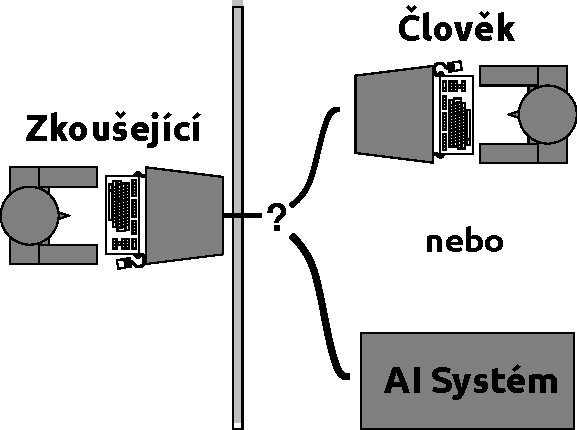
\includegraphics[width=5cm]{turing-test.pdf}
\end{center}
\end{frame}
\begin{frame}\frametitle{Jednat jako lidé --- Turingův test}
\begin{block}{}
 A. Turing: {\it Computing machinery and intelligence}, 1950
\end{block}
\begin{itemize}
 \item předpovídal, že do roku 2000 budou mít počítače 30\% šanci 5 minut šálit člověka\pause{}
 \item předjímal všechny hlavní protiargumenty, které se od té doby proti AI vyskytly\pause{}
 \item navrhl hlavní komponenty AI systémů: znalost, uvažování, porozumění (přirozenému) jazyku, učení
\end{itemize}
\end{frame}

\begin{frame}\frametitle{CAPTCHA --- Reverzní Turingův test}
\begin{center}
 
\includegraphics[width=4cm]{recaptcha-example.png}
\end{center}

 
\end{frame}


\begin{frame}\frametitle{Myslet jako lidé}
\large
\begin{center}
systém, který\\[1cm]
\begin{tabular}{c|c}
 \alert{myslí jako lidé} & myslí racionálně \\[0.5cm]
%  \noalign{\smallskip}
 \hline
%  \noalign{\smallskip} 
\\
 se chová jako lidé & se chová racionálně \\
\end{tabular}
\end{center}
\end{frame}




\begin{frame}\frametitle{Myslet jako lidé --- Kognitivní vědy}
\begin{block}{}
\begin{center}
Kognitivní vědy
\end{center}
\end{block}\pause{}
\begin{itemize}
 \item do 60. let převládal tzv. behaviorismus (lidské chování lze vysvětlit bez odkazu k ``myšlení'')\pause{}
 \item v 60. letech převládla tzv. kognitivní psychologie --- vnitřní stavy mysli jsou zásadní\pause{}
 \item je třeba model / teorie lidské mysli\hskip-1cm\pause{}
 \begin{minipage}[b]{5.6cm}
 \begin{itemize}
   \item[] Psychologie (přístup shora)\pause{}
   \begin{itemize}
     \item ``high-level''\pause{}
     \item General Problem Solver\pause{}
   \end{itemize}   
   \item[] Neurovědy (přístup zdola)\pause{}
   \begin{itemize}
     \item neuronové sítě\pause{}
     \item inteligence jako ``emergentní jev''\pause{}
   \end{itemize}
 \end{itemize}
 \end{minipage}
 \begin{minipage}[b]{4cm}
  \hskip1cm
  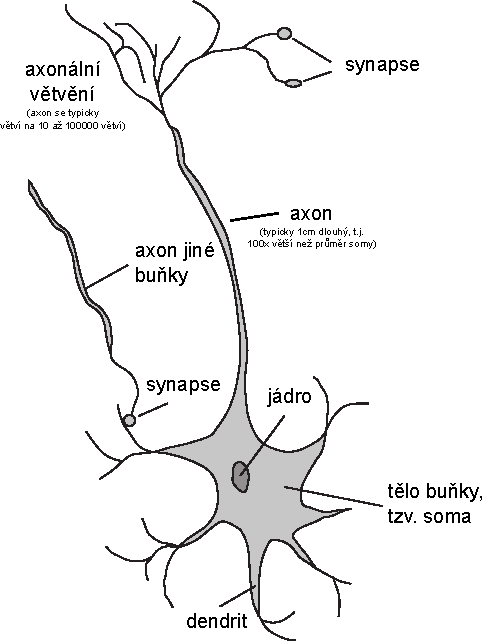
\includegraphics[height=3.4cm]{neuron.pdf}
 \end{minipage}
\end{itemize}
\end{frame}

\begin{frame}\frametitle{Myslet racionálně}
\large
\begin{center}
systém, který\\[1cm]
\begin{tabular}{c|c}
 myslí jako lidé & \alert{myslí racionálně} \\[0.5cm]
%  \noalign{\smallskip}
 \hline
%  \noalign{\smallskip} 
\\
 se chová jako lidé & se chová racionálně \\
\end{tabular}
\end{center}
\end{frame}


\begin{frame}\frametitle{Myslet racionálně --- Logika}
\begin{itemize}
 \item Aristoteles (384--322 př. Kr.): sylogismy (barbara, celarent, darii, ferio, $\dots$)\pause{}
%  bArbArA (AAA): All men are mortal, All greeks are men => All greeks are mortal.
%  cElArEnt (EAE): No gods are mortal. All greeks are gods => No greeks are mortal.
%  dArII (AII): All rabbits have fur, Some pets are rabbits => Some pets have fur.
%  fErIO (EIO): No homework is fun, Some reading is homework => Some reading is not fun.
% there are 24 valid syllogisms

%  \item Akvinský, scholastika\pause{}

 \item Leibniz (1646--1716):  calculus ratiocinator\pause{}
 \item Frege $\ldots$\pause{}
 \item (to znáte lépe)\pause{}
\end{itemize}
\begin{block}{}
\begin{center}
Problémy\pause{}
\end{center}
\end{block}
\begin{itemize}
 \item Není jasné, které z mnoha logických úsudků jsou relevantní.\pause{}
% 
 \item Není jasné, jak formalizovat problémy reálného světa, zvláště když je ve hře ``nejistota''.\pause{}
% Asi bude pršet. 
 \item Teoretické řešení $\neq$ praktické řešení.
%  Optimálně hrát šachy je z ``logického'' hlediska triviální, nicméně v praxi je toto jednoduché řešení neproveditelné
\end{itemize}


\end{frame}


\begin{frame}\frametitle{Jednat racionálně}
\large
\begin{center}
systém, který\\[1cm]
\begin{tabular}{c|c}
 myslí jako lidé & myslí racionálně \\[0.5cm]
%  \noalign{\smallskip}
 \hline
%  \noalign{\smallskip} 
\\
 se chová jako lidé & \alert{se chová racionálně}      \\
\end{tabular}
\end{center}
\end{frame}

\begin{frame}\frametitle{Jednat racionálně --- Ekonomie}
\begin{block}{}
Racionální chování je takové, které na základě dostupných informací volí akce nejpravděpodobněji vedoucí k maximalizaci ``užitku''
\end{block}\pause{}
\begin{itemize}
 \item nemusí nutně obnášet logické odvozování (reflexivní jednání)\pause{}
 \item Ekonomie --- věda o racionálním chování\pause{} (tedy nikoliv nutně o lidském chování !!)
\end{itemize}
\end{frame}

\begin{frame}\frametitle{Jednat racionálně --- Racionální agent}
\alert{Agent} je jednotka, která \emph{vnímá}\pause{} a \emph{jedná}.\pause{}
Tato přednáška je o návrhu racionálních agentů.\pause{} 
% Spoustu problémů lze formulovat jako problémy agentů: šachy: vnímá protihráčovy tahy, jedná tak, že táhne;
% ...
Abstraktně lze agenta definovat jakožto funkci z posloupností vjemů ($\mathcal P^*$) do množiny akcí ($\mathcal A$):
\begin{block}{}
\begin{displaymath}
 f: {\mathcal P}^* \to {\mathcal A}
\end{displaymath}
\end{block}
\end{frame}


\begin{frame}\frametitle{Trocha historie}
\begin{itemize}
 \item[43] booleovský model neuronových sítí (McCulloch, Pitts) [ekvivalence Turingova stroje a neuronové sítě]\pause{}
 \item[47] Turing přednáší o AI na setkání Londýnské matematické společnosti\pause{}
 \item[50] SNARC --- první umělá neuronová síť, 40 neuronů (Minsky, Edmonds)\pause{}
  \begin{block}{}
  \small
 Minsky napsal v Princetonu dizertaci o neuronových sítích a výpočtech. Komise byla skeptická, že to není matematika,
 nicméně von Neumann prý řekl, že pokud to není nyní, tak jednou bude.
 \end{block}\pause{}
 \item[50] Turing: {\tt Computing Machinery and Intelligence}
 \end{itemize}
\end{frame}

\begin{frame}\frametitle{Trocha historie}
 \begin{itemize}
 \item[56] Workshop v Dartmouth (McCarthy, Minsky, Shannon, ...), Logic Theorist (Newell, Simon z CMU)\pause{}
 \begin{block}{}
  \small
  Logic Theorist brzy dokázal většinu vět z druhé kapitoly Russelových Principií a v jednom případě našel i kratší důkaz.
  Russell byl potěšen, nicméně editoři časopisu {\it J. of Symbolic logic} už tak potěšení nebyli a článek spoluautorů
  Newella, Simona a Logical Theorist zamítli. 
 \end{block}\pause{}
 \item[56--59] 
 \begin{itemize}
   \item[] General Problem Solver (nástupce Logical Theorist)\pause{}
   \item[] Geometry Theorem Prover (IBM, 1959)\pause{}
   \item[] Samuel: Počítačová dáma, postupně se dostala na úroveň silného amatéra (počítač brzy hrál lépe než Samuel)\pause{}
   \item[] McCarthy: Lisp (MIT), {\it Programs with Common Sense} --- reprezentace znalostí v AI\pause{}
   \item[] Slagle: SAINT uměl integrovat typické příklady prvního ročníku analýzy, Evans: ANALOGY uměl řešit příklady
           na ``analogii'' z IQ testů, mikrosvěty (SHRDLU)\pause{}
 \end{itemize}
 \item[65] Rezoluce (Robinson)
\end{itemize}
\end{frame}
\begin{frame}\frametitle{Trocha historie}
\begin{itemize}
 \item[66--74] Skoro úplně vymizel výzkum neuronových sítí\pause{}, návrat do reality\pause{}
 \begin{block}{}
 \small
 The spirit is strong but the flesh is weak $\Rightarrow$
Russian %  спирт, конечно, готов, но мясо протухло 
 $\Rightarrow$ The vodka is good but the meat is rotten.\pause{}(pravděpodobně hoax)
 \end{block}\pause{}

 \item[69-79] První znalostní systémy (DENDRAL --- interpretace spekter)\pause{}
 \item[80-93] ``The Decline and Fall of Expert Systems''\pause{}
 \item[85--] Návrat neuronových sítí\pause{}
 \item[95--] Agenti, agenti, agenti ...
\end{itemize}
\end{frame}

\begin{frame}\frametitle{Aktuální stav --- State of the Art}
\begin{block}{}
\begin{center}
 Co dovede AI dnes?
\end{center}
\end{block}

\begin{itemize}
 \item[] Hrát obstojně stolní tenis\pause{}\hfill\yes\pause{}
 \item[] Řídit bezpečně auto po točité horské silnici\pause{}\hfill\yes\pause{}
 \item[] Řídit bezpečně auto na magistrále.\pause{}\hfill\no/\yes\pause{}
 \item[] Překládat mluvenou angličtinu do mluvené švédštiny v reálném čase\pause{}\hfill to závisí\pause{}
 \item[] Hrát Go na profesionální úrovni\pause{}\hfill\no\pause{}
%  \url{http://www.wired.com/wiredscience/2009/03/gobrain/} (přečíst komentáře)
 \item[] Přijít na fyzikální zákony\pause{}\hfill\yes\pause{}
 \begin{itemize}
   \item[] \url{www.wired.com/wiredscience/2009/04/newtonai/}
   \item[] \url{www.wired.com/wiredscience/2009/04/robotscientist/}
 \end{itemize}\pause{}
 \item[] Hodinu si úspěšně povídat s člověkem\pause{}\hfill\no\pause{}
 \item[] Vymyslet (úmyslně) vtipný příběh.\pause{}\hfill\no\pause{}
\end{itemize}
\end{frame}

\begin{frame}\frametitle{DARPA Grand Challenge}
\begin{itemize}
 \item[2004] Mojave Desert\pause{}, 240 km\pause{}, 15 vozidel\pause{}, nejlepší skončil po 11 km\pause{}
 \item[2005] Beer bottle pass\pause{}, několik tunelů\pause{}, 23 vozidel\pause{}, 5 dokončilo !\pause{}
\end{itemize}
\begin{block}{}
\url{http://www.youtube.com/watch?v=TDqzyd7fDRc}
\end{block}\pause{}
\begin{itemize}
 \item[2007] Urban challenge, George Air Force Base\pause{}, 96 km\pause{}, 11 vozidel se kvalifikovalo\pause{},  6 dokončilo !
\end{itemize}
\end{frame}


\begin{frame}\frametitle{DARPA Grand Challenge}
\begin{center}
\url{http://www.youtube.com/watch?gl=CZ&v=M2AcMnfzpNg} 
% \movie[width=6.4cm,height=3.6cm]{\url{http://www.youtube.com/watch?gl=CZ&v=M2AcMnfzpNg}}{darpa.mp4}
\end{center}
\end{frame}


\begin{frame}\frametitle{Další $\ldots$}
\begin{itemize}
 \item RoboCup\pause{}
 \item Curiosity\pause{}
 \item $\ldots$
\end{itemize}
\end{frame}






% \begin{frame}\frametitle{References}

% \begin{thebibliography}{}
% \bibitem[Kun78]{WeakPp}
% Kunen, K.,  \emph{{Weak $P$-points in $N^*$}}, vol. {Proc. Bolyai J\'anos Soc. Colloq. on Topology}, pp.~741--749, 1978.
% 
% \bibitem[vD93]{Douwen}
% Douwen, E. K. van, \emph{Applications of maximal topologies}, Topology Appl., \textbf{51} (1993),  125--139
% 
% \bibitem[DGS88]{Dow}
% Dow, A., Gubbi, A. V. and Szymański, A., \emph{Rigid Stone spaces within ZFC}, Proc. Am. Math. Soc. \textbf{102} (1988), no.~3, 745--748.
% 
% \bibitem[vM82]{Mill16}
% Mill, J. van, \emph{{Sixteen types in $\beta\omega-\omega$}}, Topology Appl. \textbf{13} (1982), 43--57.
% 
% \bibitem[Sim85]{SimonIndep}
%  Simon, P. \emph{Applications of independent linked families}, Colloq. Math. Soc. {J\'anos} Bolyai \textbf{41} (1985), 561--580.
% 
% \bibitem[Ver07]{Verner}
%  Verner, J. L., \emph{Lonely points in $\omega^*$}, Topology Appl., \textbf{155} (2008),  1766--1771
% 
% 
% \end{thebibliography}
% \end{frame}

\end{document}


